\documentclass[font=default]{mpltx}
\usepackage{bm, ctex, array}
\usepackage{subfigure}
\usepackage{multirow}
% 以下至 \begin{document} 都仅是本文件为了方便额外定义的命令, 写报告时不需要.
\hypersetup{colorlinks=false}% 超链接带颜色
\usepackage{xcolor}
% 以上是本文件为了方便额外定义的命令, 写报告时不需要.
\linespread{1.5}
\begin{document}

\title{扫描隧穿显微镜} % 切合报告内容, 简短明确, 可以不同于讲义
\author{MaskedName} % 这里 \emailphone 一定要紧跟在 \author 后方
\emailphone{MyMail@stu.pku.edu.cn}{Tel}
% 如果改用 \email 则仅需要邮箱参数
\affiliation{北京大学物理学院\quad 学号: StudentID}
\date{\zhdate{2024/11/28}}
\begin{abstract}
  本实验利用扫描隧道显微镜(STM)对高定向热解石墨(HOPG)样品进行了原子级分辨率的表面成像,以直观验证量子隧穿效应并探索STM在表面分析中的应用。通过精确控制STM探针与样品之间的距离,我们成功捕获了样品表面的原子结构图像。此外,通过比较STM 所成图像与样品实际结构,粗略地校准了STM的探针控制系统。本研究不仅加深了对量子隧穿效应的理解,也为STM技术在材料科学、电子学和纳米技术等领域的应用提供了实验基础和理论支持。
\end{abstract}
\keywords{扫描隧穿显微镜(STM),高定向热解石墨(HOPG),隧穿效应,压电系数}

\maketitle

\section{引言}
在量子力学的理论下,微观粒子有一定概率穿透高于其总能量的势垒,这一现象被称为隧穿效应。根据这一原理,在1981年,IBM苏黎世实验室的两位科学家Binnig和Rohrer发明了扫描隧穿显微镜(Scanning Tunneling Microscope, STM),并因此获得了1986年的诺贝尔物理学奖。STM是一种利用量子力学的隧穿效应来实现原子尺度的成像的显微镜,它可以在原子尺度上观察到物质的表面形貌。STM平行于表面(横向)的分辨率可以达到0.1nm,而垂直表面(纵向)的分辨率能够高于1Å,是目前最高分辨率的显微镜之一,被广泛应用于表面物理、表面化学、材料科学等领域。

本次实验中,我们通过STM观察高定向热解石墨(Highly Oriented Pyrolytic Graphite, HOPG)的表面形貌,了解STM的基本原理和工作原理,掌握STM的操作方法,熟悉STM的工作特性,以及学习STM的应用。此外,我们会考察压电材料在STM中的关键作用,并且通过实验标定$x,y$方向陶瓷的压电系数。

\section{理论\cite{book}}
考察定态薛定谔方程:
\begin{equation}
  \left[ -\frac{\hbar^2}{2m} \nabla^2 + V(\bm{r}) \right] \psi(\bm{r}) = E \psi(\bm{r}).
\end{equation}
在$V(r)>E$的区域,波函数$\psi(\bm{r})$不一定为零(如果$V$不是无穷大的话),因此入射粒子要穿透一个$V(r)>E$的有限区域的几率是不为零的,这就是量子隧穿效应。

为了估计隧穿几率,我们可以考虑一维的定态薛定谔方程:
\begin{equation}
  -\frac{\hbar^2}{2m} \frac{d^2\psi(x)}{dx^2} + V(x) \psi(x) = E \psi(x).
\end{equation}
再考虑一个有限高度的方势垒,其形式为:
\begin{equation}
  V(x) = \begin{cases}
    0, & x < 0, x > s, \\
    \phi, & 0 < x < s.
  \end{cases}
\end{equation}
其中入射波、反射波、透射波的形式分别写作:$e^{ikx},\ Re^{-ikx},\ T^{ikx}$,其中$k=\sqrt{2mE}/\hbar$;在$0<x<s$区域内波函数并不为零,而是具有指数衰减的形式:
\begin{equation}
  \psi(x) \propto e^{-\kappa x},\ \kappa = \sqrt{\frac{2m(\phi-E)}{\hbar^2}}\approx \sqrt{\frac{2m\phi}{\hbar^2}}.
\end{equation}
加入边界条件进行求解,我们最终可以得到隧穿电流的表达式
\begin{equation}
  \frac{I}{I_0}=|T|^2\propto e^{-2\kappa s}.
\end{equation}
这里$\phi$为有效平均势垒高度,$s$为势垒有效宽度。我们可以看到,隧穿电流随着势垒高度的增加而指数衰减,在工作状态下,$s$每改变0.1nm,隧穿电流就会改变一个量级。这自然导致了STM的高分辨率。隧穿电流的密度分布如\autoref{fig:current} 所示。
\begin{figure}
  \centering
  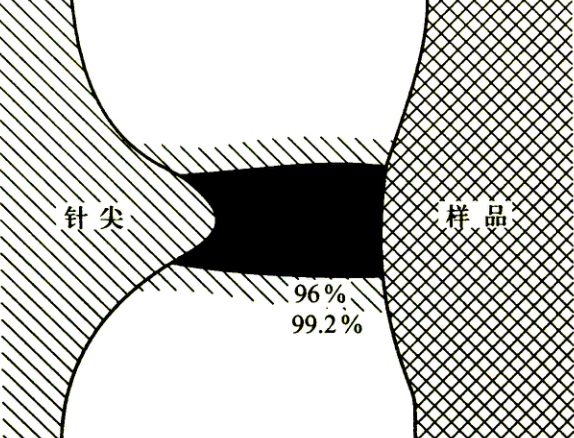
\includegraphics[width=0.4\textwidth]{fig/current.png}
  \caption{计算得到的从针尖到表面的隧穿电流分布图}
  \label{fig:current}
\end{figure}

根据隧穿电流的这一特性,我们在STM可以将针尖装在压电陶瓷构成的三维扫描架上,通过改变压电陶瓷的电压来控制针尖位置,并且在针尖和样品之间加上偏置电压$V_b$。工作时,我们在$x,y$方向向压电陶瓷施加扫描电压,就可以让针尖在样品表面移动。STM一般有两种工作模式:恒流模式和恒高模式。在恒流模式下,我们保持隧穿电流$I$不变,通过调节$z$方向陶瓷上的电压控制针尖高度,从而实现对样品表面的成像。在恒高模式下,我们保持针尖和样品之间的距离$z$不变,通过记录隧穿电流的大小得到关于表面的信息。本实验中,我们使用恒流模式进行成像。

\section{实验内容}
本实验使用的STM工作原理如\autoref{fig:stm} 所示。实验中,成像区域的定位通过压电陶瓷实现,其外加电压和伸长量之间的关系为:
\begin{equation}
  \Delta L = cV
\end{equation}
这里的$c$称为压电系数。因此,我们在实验中使用的坐标可以用电压表示。
\begin{figure}
  \centering
  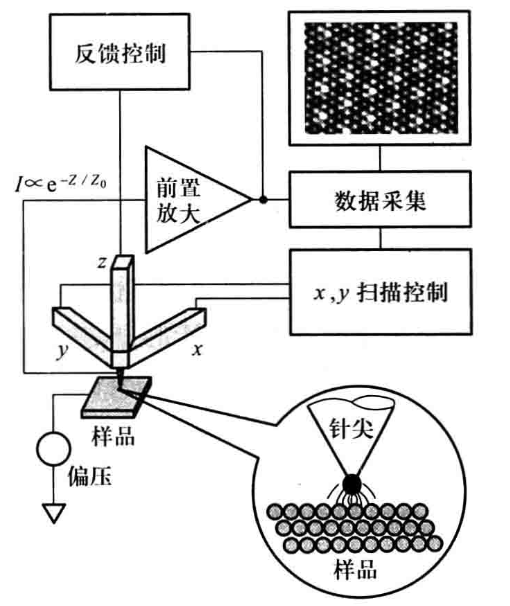
\includegraphics[width=0.4\textwidth]{fig/stm.png}
  \caption{STM工作原理示意图}
  \label{fig:stm}
\end{figure}

STM的针尖由实验室提供,实验过程中,我们可以通过在针尖和样品之间加正负2.5 V的脉冲电压(已经编写在控制程序中),使针尖处于场发射的状态,以清洁和锐化针尖。但是由于在这个过程中,会发生针尖和样品间物质的转移,所以处理过程中针尖应该尽量避开正在观察的表面。

用STM成像步骤如下:
\begin{itemize}
  \item \textbf{初始设置}:操作控制面板上的旋钮,将X和Y电压的起点(ORIGIN)设定为0 V,并将其变化范围(RANGE)扩展至最大值200 V。同时,将隧穿电流$I$预设在大约1 nA左右,初始扫描时间设置为2000 ms。
  \item \textbf{自动进针}:在控制程序上进行自动进针操作,直到仪器发出警告声,说明已经有非零的隧穿电流产生。此时手动进针,直到$z$方向陶瓷上的电压达到90 V。之后点按20次手动退针,STM即进入工作状态。
  \item \textbf{开始扫描}:设置偏置电压$V_b$之后开始进行扫描,此时会在电脑端上同步显示扫描的结果,通过调整A/D INPUT面板中的信号增益(AMPLIFICATION)和信号偏置(OFFSET)来调整成像效果,使得信号波形能被完整的记录下来。
  \item \textbf{调整参数}:寻找样品中较为平整的一块,调整ORIGIN和RANGE进行扫描,同时也可以修改隧穿电流、偏置电压和扫描时间,使得成像效果最好。
  \item \textbf{自动退针}:在实验结束后,在控制程序上进行自动退针操作,随后关闭仪器电源和程序。
\end{itemize}

\section{实验结果与分析}
\subsection{石墨的原子分辨像}
首先我们进行大范围扫描,选取图像中的平坦区域,一步步虽小$x,y$扫描范围、调整扫描起点,以获得更佳精确的扫描图像。同时我们在缩小扫描范围的过程中,也要适当的减小扫描时间,以保证成像的清晰度。最终我们获得了如\autoref{fig:stm_photos} 所示的HOPG的原子分辨像。
\begin{figure}
  \centering
  \subfigure[扫描范围$200\times200$ V]{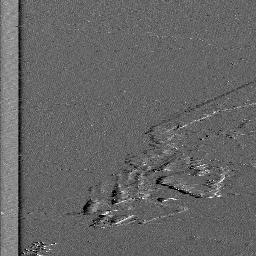
\includegraphics[height=0.4\textwidth]{fig/stm_photos/200x200_2000ms_amp20_bias926_tc1.04.jpg}}
  \subfigure[扫描范围$100\times100$ V]{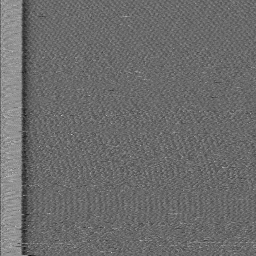
\includegraphics[height=0.4\textwidth]{fig/stm_photos/100x100_1000_20_926_1.04.png}}
  \subfigure[扫描范围$40\times40$ V]{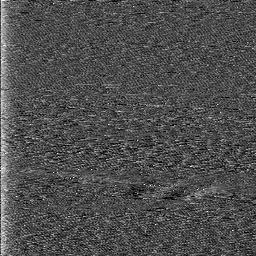
\includegraphics[height=0.4\textwidth]{fig/stm_photos/40x40_700_50_926_1.04.jpg}}
  \subfigure[扫描范围$10\times10$ V]{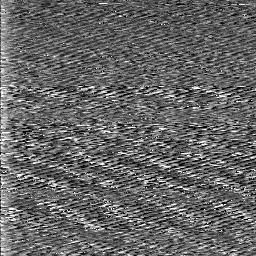
\includegraphics[height=0.4\textwidth]{fig/stm_photos/10x10_500_100_926_1.04.jpg}}
  \subfigure[扫描范围$4\times4$ V]{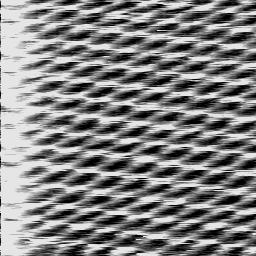
\includegraphics[height=0.4\textwidth]{fig/stm_photos/'4x4_150_100_300_1.32'.jpg}}
  \subfigure[扫描范围$2\times2$ V]{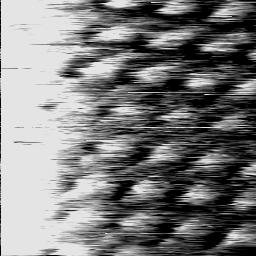
\includegraphics[height=0.4\textwidth]{fig/stm_photos/2x2_50_100_550_1.00.jpg}}
  \caption{石墨(HOPG)在不同STM参数下的原子分辨像}
  \label{fig:stm_photos}
\end{figure}

不同图像对应的STM参数如\autoref{tab:stm_params} 所示。我们可以看到,随着扫描范围的缩小,我们可以获得更高分辨率的图像(在$10\times10$的图像中,我们已经可以隐约看到原子的像了),但是同时也需要适当减少扫描时间和增大信号放大倍数,以保证成像的清晰度。在$4\times4$和$2\times2$的图像中,我们就可以清晰地看到石墨表面的原子结构了。
\begin{table}[]
  \label{tab:stm_params}
  \caption{不同图像对应的STM参数列表}
  \vspace{0.2cm}
  \begin{tabular}{c|cc|c|c|c|c}
    \hline
  图像 & \multicolumn{2}{c|}{范围(RANGE/V)} & 隧穿电流/nA & 偏置电压/V & 扫描时间/ms & AMPLIFICATION \\
     & $x$     & $y$   &         &        &         &             \\\hline
  a  & 200     & 200 & 1.04    & 1000   & 2000    & 20            \\
  b  & 100     & 100 & 1.04    & 1000   & 1000    & 20            \\
  c  & 40      & 40  & 1.04    & 1000   & 700     & 50            \\
  d  & 10      & 10  & 1.04    & 1000   & 500     & 100           \\
  e  & 4       & 4   & 1.32    & 300    & 150     & 100           \\
  f  & 2       & 2   & 1.00    & 500    & 50      & 100           \\\hline
  \end{tabular}
\end{table}

可以看到,扫描的范围越小,我们设定的扫描时间也越短,这是因为如果扫描时间过长,针尖会产生比较严重的热漂移,从而导致没有办法成清晰的像。同时我们在扫描范围缩小的时候,也将偏置电压适当减小,在更小的电压下保持同样的隧穿电流就需要更短的针尖-样品距离,从而可以使针尖运动更加灵敏,成像更加清晰。
\subsection{标定$x,y$陶瓷的压电系数}
已知HOPG的原子分辨像中,两个原子之间的距离为0.246 nm,我们可以通过测量图像中两个原子之间的距离,来标定$x,y$陶瓷的压电系数。如\autoref{fig:2x2} 所示,在$2\times2$ V的图像中,包含有12个左右原子的距离,于是我们可以根据压电陶瓷的线性关系估计得到压电系数:
\begin{equation}
  c_x\approx c_y\approx \frac{12\times0.246\ \text{nm}}{2\ \text{V}}\approx1.5\ \text{nm/V}.
\end{equation}
\begin{figure}
  \centering
  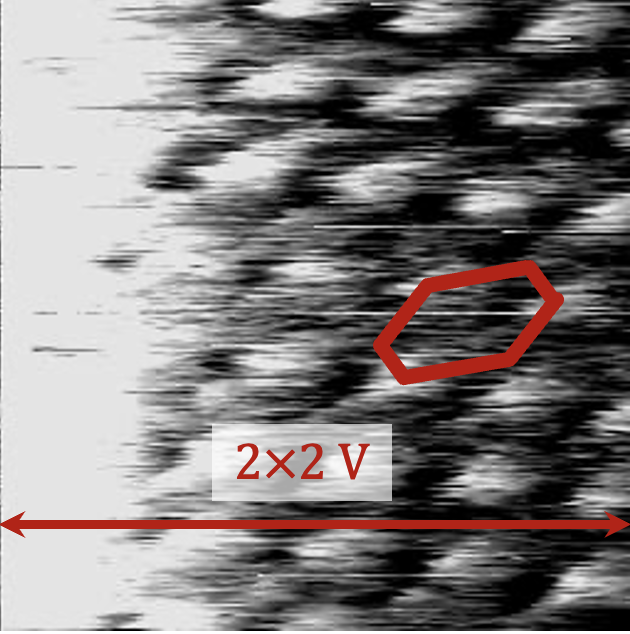
\includegraphics[width=0.4\textwidth]{fig/2x2.png}
  \caption{石墨(HOPG)在$2\times2$ V的原子分辨像,其中一个六边形用红线标出,两个原子之间的距离为0.246 nm}
  \label{fig:2x2}
\end{figure}

这里需要说明的是,上面给出的压电系数仅仅只是一个粗略的估计,由\autoref{fig:2x2} 中六边形的畸变可以看出,样品表面和针尖不是完全垂直的,但是,成像时发生的热漂移也会导致图像的畸变,从而造成我们计算的不准确。

\section{结论}
本实验通过STM对高定向热解石墨(HOPG)进行成像,通过对不同范围的扫描,我们最终实现了原子级别的分辨像。同时,我们也通过测量图像中的原子间距,估计了$x,y$陶瓷的压电系数$c_x\approx c_y\approx1.5$ nm/V,这有助于我们对其他材料成像的过程中得知材料中原子之间的距离。此次实验中获得的原子级分辨率图像为量子隧穿效应和原子理论提供了最坚实的证据。该技术凸显了精确控制和精细测量的关键性,这些也是实现技术突破的主要挑战;同时,扫描隧道显微镜(STM)的直观性也展现了其巨大的潜力,预示着扫描探针显微技术将在科学研究和纳米制造技术中扮演越来越重要的角色。

\section{致谢}
感谢季航老师在实验中的细致指导和耐心帮助。
\begin{thebibliography}{}
  \bibitem{book} 吴思诚, 荀坤. 近代物理实验(第四版)[M]. 北京: 高等教育出版社, 2015.
\end{thebibliography}

\appendix

\section{思考题}
\subsection{HOPG的院子排列为六角密排(无心的),为什么我们在实验中看到的HOPG的原子分辨像是有心的六角密排?}
\begin{figure}
  \centering
  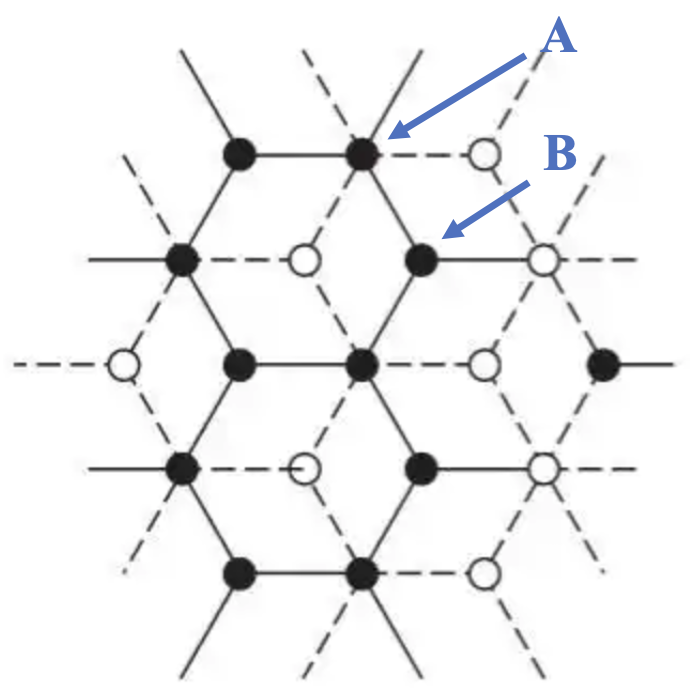
\includegraphics[width=0.4\textwidth]{fig/HOPG_struct.png}
  \caption{石墨(HOPG)的原子排列示意图}
  \label{fig:HOPG_struct}
\end{figure}
如\autoref{fig:HOPG_struct} 所示,石墨表层的原子可以分为两类:A类原子的下方正对着下层原子,而B类原子的下方是下层空隙。这导致对于A类原子来说,两层原子的电子云($\pi$键)发生重叠,这导致A类原子的电子云向内部集中;而对于B类原子来说,空隙会使得电子云拥有更大的活动空间,因此分布更为分散。这样,在STM的成像中,两种原子在图像上表现出的“高度”不同。事实上,对比\autoref{fig:2x2} 中的图像,我们可以看到,A、B类原子分别对应图像中的黑、白点。如果只看A或者B类的原子,自然会出现有心的六角密排。

\end{document}
